% CIPHER manuscript body. Shared by the named and anonymous builds. Every corpus and result number is a macro from
% generated/*.tex (written by analysis/corpus_stats.py, analysis/labelfree.py and analysis/exploratory.py); design
% constants are stated in text.
\newif\ifresults
% Generated by analysis/corpus_stats.py from data/cases/manifest.json. Do not edit.
\newcommand{\NFrame}{237}
\newcommand{\NRetrieved}{30}
\newcommand{\NSnapshotEligible}{24}
\newcommand{\NPairEligible}{12}
\newcommand{\NEvalRepos}{8}
\newcommand{\NEvalReposWord}{eight}
\newcommand{\NCalRepos}{2}
\newcommand{\NCalReposWord}{two}
\newcommand{\NCalOriginals}{7}
\newcommand{\NCalVariants}{7}
\newcommand{\NOriginals}{27}
\newcommand{\NVariants}{27}
\newcommand{\NControls}{27}
\newcommand{\NEvalContexts}{81}
\newcommand{\NAnnotated}{54}
\newcommand{\NRelAncestor}{16}
\newcommand{\NRelUnrelated}{5}
\newcommand{\NRelSameFile}{6}
\newcommand{\NVarTarget}{16}
\newcommand{\NVarPlacement}{11}
\newcommand{\NEvalAgentsFiles}{117}

% Generated by analysis/results.py. Results pending.
\newcommand{\ResultsHeadline}{results once the human reference labels are final.}
\newcommand{\ResultsSection}{\textbf{Pending.} Human reference labels are not final, so no accuracy is reported. Held-out model runs are sealed.}
\newcommand{\AbstractText}{\textbf{Draft: results pending human reference labels.}}
\newcommand{\ConclusionText}{Pending.}
\newcommand{\AIDisclosure}{Pending.}

\IfFileExists{generated/exploratory.tex}{% Generated by analysis/exploratory.py (exploratory, post-hoc). Do not edit.
\newcommand{\RepeatIdentical}{81}
\newcommand{\RepeatDiffTotal}{13}
\newcommand{\RepeatDiffOrig}{3}
\newcommand{\RepeatDiffVar}{4}
\newcommand{\RepeatDiffCtrl}{6}
\newcommand{\BOnePDCitesOffChain}{21}
}{}

\title{CIPHER: Contextual Instruction Precedence and Hierarchy Evaluation for Repositories}

\ifanon
\author{\IEEEauthorblockN{Anonymous Authors}\IEEEauthorblockA{Affiliation withheld for review}}
\else
\author{\IEEEauthorblockN{Awaiz Ahmed}\IEEEauthorblockA{Al Ain University\\United Arab Emirates\\202310183@aau.ac.ae}
\and
\IEEEauthorblockN{Mohammad Umar}\IEEEauthorblockA{Al Ain University\\United Arab Emirates\\202240077@aau.ac.ae}
\and
\IEEEauthorblockN{Huda Mueen}\IEEEauthorblockA{Al Ain University\\United Arab Emirates\\Hudamueen2407@gmail.com}}
\fi

\maketitle

\begin{abstract}
\ifresultsRepository instruction files such as AGENTS.md guide AI coding agents, and a nested file may legitimately refine or
replace guidance from its ancestors, so an apparent disagreement is not necessarily a defect. CIPHER defines a
task-conditioned classification of instruction pairs under a declared directory-precedence profile into five labels:
unresolved conflict, valid override, disjoint applicability, compatible, and insufficient evidence. From a public
configuration dataset we built a traceable pilot set of \NOriginals{} real instruction pairs from \NEvalReposWord{}
repositories at pinned commits, each with a context-changing variant and an order control, and a blinded
annotation protocol. Human reference labels have not yet been collected, so this short paper reports a
preliminary analysis, frozen by hash before predictions were opened, that needs none: accuracy on the \NPDMain{}
originals and variants whose label the profile fixes from file paths, and label-free measures elsewhere. With one local
open-weight model, a direct prompt given the full evidence and a structured pipeline that computes applicability and
precedence explicitly were both correct on all \NPDMain{} profile-determined cases, whereas a keyword heuristic flagged
\BZeroPDFalseConf{} of \NPD{} such cases as conflicts. No model judged any original or variant to be an unresolved
conflict; the methods disagreed mainly on condition-based applicability, and swapping only the order of the two
instructions changed 4 of \NControls{} predictions for each model arm. The structured pipeline used more output tokens
than the direct prompt (\BTwoMeanOut{} versus \BOneMeanOut{} per case) without a measurable gain. Human labels for the
semantic cases are the next step.
\else\textbf{Draft: results pending human reference labels.}\fi
\end{abstract}

\begin{IEEEkeywords}
AI coding agents, AGENTS.md, instruction conflicts, repository mining, scope and precedence
\end{IEEEkeywords}

\section{Introduction}\label{sec:intro}
AI coding agents read project guidance from natural-language files in the repository. The AGENTS.md convention allows
one file per package and states that ``the closest AGENTS.md to the edited file wins''~\cite{agentsmd}. Apparent
disagreement between such instructions is therefore not always a defect. Take two rules, ``use exactly four spaces per
indentation level'' and ``use exactly two''. If both sit in the root file, they genuinely conflict for any new line; if
the second sits in \texttt{web/AGENTS.md}, it is a documented local override for \texttt{web/src/button.ts}; and if it
sits in \texttt{api/AGENTS.md}, it does not apply to that target at all. The wording is identical in all three
situations; only the files' placement relative to the task's target differs.

A conflict detector can fail in both directions: it can miss incompatible obligations, or it can report a legitimate
local exception as a defect and suggest deleting useful guidance. The two AGENTS.md detectors we examined flag
contradictions from text alone. In a study of 100 repositories, a model-based smell detector, which reads one file at a
time, reported 28 conflicting-instruction cases, of which manual analysis by that study's first author confirmed
16~\cite{santos2026smells}; the keyword heuristics of Ruleherd~\cite{ruleherd} compare files without regard to scope. We
found no study that tests whether explicit scope and precedence reduce such false alarms.

CIPHER asks whether making applicability and precedence explicit improves the classification of apparent conflicts:
how reliably humans separate the labels (RQ1), whether a structured pipeline beats a direct model given the same
evidence (RQ2), and whether predictions respond correctly to relevant context changes and stay stable under irrelevant
ones (RQ3). We contribute (1)~a task-conditioned, five-label definition of the problem under a declared AGENTS.md
loading profile; (2)~a traceable pilot set of \NOriginals{} real instruction pairs from \NEvalReposWord{} repositories at
pinned commits, each with one context-changing variant and one order control, and an annotation protocol and tool
designed for blinded labeling (not yet used) for RQ1; and (3)~a comparison of a keyword heuristic, a direct model given
an evidence packet, and a structured pipeline given the same packet and model. Human labels have not yet been collected, so Section~\ref{sec:results} reports
\ifresultsa preliminary analysis without human labels: on cases whose label the profile fixes from directory structure, a direct
model given the full evidence was already correct, so the structured pipeline added cost without measurable benefit
there, while the methods disagreed on condition-based applicability.\else results once the human reference labels are final.\fi{} The protocol, data,
prompts, raw outputs, and analysis code are released\ifanon{} (anonymized artifact link withheld)\else{} at
\url{https://github.com/4waiz/cipher}\fi.

\section{Related Work}\label{sec:related}
Context files have been characterized at scale~\cite{chatlatanagulchai2026agentreadmes,galster2026dataset}, and their
effect on task success is contested~\cite{gloaguen2026evaluating}. Configuration Smells~\cite{santos2026smells} treats
conflicting instructions within one file as a smell; Context Rot~\cite{treude2026contextrot} studies staleness.
WIRE~\cite{yan2026wire} grounds rules in spans and models activation conditions, without matched compatible-pair or
priority controls. ContextCov~\cite{sharma2026contextcov} extracts and enforces scoped constraints;
OctoBench~\cite{ding2026octobench} measures which source an agent follows under explicit conflicts.
Guidefold~\cite{guidefold} already resolves guidance with a most-specific-scope lattice, noting that human-labeled
conflicts were still missing. Injected cross-file contradictions had no detectable effect on adherence
in~\cite{mcmillan2026adherence}, and Arbiter catalogs interference in system prompts~\cite{mason2026arbiter}.
Applicability and precedence reasoning are therefore not new; our contribution is a task, a traceable set of mined
AGENTS.md pairs with controlled variants, and a same-evidence comparison of a direct and a structured model.

\section{Task and Instruction Profile}\label{sec:task}
A \emph{case} is one pair of verbatim instruction spans (with file path, line numbers, heading, and enclosing section),
one concrete task that edits one target file, one pinned commit, and one loading profile. The label concerns this pair
and task, not the overall quality of a repository.

\textbf{Profile P1} (frozen; an experimental interpretation of~\cite{agentsmd}, not a claim about every tool). Only
AGENTS.md files participate. The binding loaded set is every AGENTS.md on the target's ancestor directory chain; files
in unrelated branches are not loaded. A loaded instruction is in force unless its own wording limits it. When two loaded
instructions are incompatible on the same decision, the more deeply nested file wins, and ancestor instructions about
other decisions stay in force. Equal authority (same file or same depth) is not ranked by order of appearance; only an
explicit statement can create priority. User prompts, other file formats, imports, symbolic links, multiple working
roots, and multi-target tasks are excluded.

\textbf{Labels and decision sequence.} The handbook orders the judgment as follows: (1)~if meaning or applicability
cannot be established, \emph{Insufficient evidence}; (2)~if, before priority, either instruction is inactive (not
loaded, or excluded by its own condition), \emph{Disjoint applicability}; (3)~if the active instructions can be
satisfied together, \emph{Compatible} (different decisions, refinements, duplicates, or a preference beside a
requirement); (4)~otherwise \emph{Valid override} if P1 or an explicit statement picks a winner, else
\emph{Unresolved conflict}. Modality is preserved: ``prefer X'' does not forbid Y, and descriptions or examples are not
rules unless worded as requirements.

\section{Corpus and Annotation Protocol}\label{sec:corpus}
\textbf{Sampling.} The frame was the \texttt{context\_files.csv} table of a public configuration
dataset~\cite{galster2026dataset} (Zenodo 20090356): \NFrame{} repositories with a root and a nested AGENTS.md. In a
seeded random order we retrieved the first \NRetrieved{} through the GitHub API at their default-branch commit on
21~October~2026, storing every AGENTS.md as inert JSON with its SHA-256. Repositories needed an open-source license, no
fork or archive status, an untruncated Git tree, no symlinked AGENTS.md, and a root and a nested file with five or more
non-empty lines (\NSnapshotEligible{} of \NRetrieved{}). Files under template, example, vendored, or hidden directories
were excluded as separate project roots.

\textbf{Candidate pairs.} Retrieval is separate from classification and challenge-oriented: directive units (list items
and paragraphs outside code fences) are paired when they share a specific tool, command, or convention term or name
different values from one family (e.g., \texttt{npm} and \texttt{pnpm}); the score favors different values, opposite
polarity, conditions, and precedence words, and verbatim duplicates are excluded. Of the repositories with at least four
pairs, two across files (\NPairEligible{}), the first \NCalReposWord{} in frame order formed the calibration split and
the next \NEvalReposWord{} the evaluation split. Up to four pairs per repository were selected by score with relation
quotas, yielding \NOriginals{} evaluation originals (\NRelAncestor{} ancestor--descendant, \NRelUnrelated{}
unrelated-branch, \NRelSameFile{} same-file) and \NCalOriginals{} calibration originals. Tasks come from fixed templates
written with AI assistance (e.g., ``make a small fix in \texttt{<target>} and complete the checks this change requires
before committing''); targets are real files. The sample cannot estimate how often conflicts occur.

\textbf{Strata.} Each original has a \emph{context-changing variant} that keeps both instructions' wording and changes
one documented property: the target path (\NVarTarget{} cases, moving the target outside the nested file's directory)
or the placement of one instruction (\NVarPlacement{} cases, relocating it to the root or to a nested file on the
target's chain). A relocated instruction is appended under a copy of its nearest heading, so outer headings of its
original file are lost; no human has yet checked whether this changes meaning. Each original also has an
\emph{order control} that only swaps the presentation order of the two instructions. Variants and controls are
constructed material; every result states how many cases come from each stratum.

\textbf{Annotation protocol (prepared, not yet used).} A frozen handbook and an offline tool support two independent
annotators and an adjudicator, with separately randomized packets, opaque item IDs, no predictions or strata, the
target's directory chain marked, full files, and a \NCalItems-item calibration packet (\NPracticeWord{} invented
practice items). No human labels were collected for this submission, so RQ1 is not answered here.

\section{Methods and Setup}\label{sec:methods}
\textbf{B0} applies Ruleherd's contradiction rules (v0.1.3, commit 94559fc6: keyword pairs such as npm/pnpm and
never/always polarity across different files) to the two spans and yields a binary flag. \textbf{B1} is one call that
receives the evidence packet (task, target, commit, all AGENTS.md paths, both spans with line-numbered sections, scope
statements), the profile, the label definitions, and the decision sequence, but not the full files or the chain
marking. \textbf{B2}, the CIPHER pipeline, uses the same model and packet: one call extracts each instruction's
requirement, decision, modality, explicit condition, and whether that condition covers the task, plus any explicit
priority statement; code computes the loaded set and depth precedence (an unclear condition counts as covering the
task; B2 cannot abstain); a second call, made only when both instructions stay active and neither is merely
descriptive, judges incompatibility; fixed rules map the results to a label. \textbf{B1R}, an equal-call control, is
B1 followed by one self-review call.

All arms used the open-weight Qwen3.6-35B-A3B~\cite{qwen36} (3B active parameters; Q4\_K\_M; Ollama digest a7eb95c5,
served by Ollama 0.40.6, auto-updated to 0.40.7 before the last four B2 cases and B1R) on one laptop GPU with thinking
enabled, the model card's settings for precise coding (temperature 0.6, top-$p$ 0.95, top-$k$ 20), a fixed seed,
JSON-schema output, and up to two retries. Requests contained only the method prompt and the evidence. Before any
held-out run, calibration led to one change (B2's sufficiency field became a two-value enum); before any held-out output
was opened, an independent AI code review found that the scope-statement header implied all listed files were loaded,
so it was corrected and all runs repeated. Inputs, prompts, and schemas were frozen by hash before the reported runs,
which stayed sealed until the analysis was frozen. The planned primary outcome, macro-F1 against human labels, could not
be computed; a plan addendum written before the predictions were opened defines the reported analysis.

\section{Results}\label{sec:results}
\ifresults\begin{table*}[t]
\caption{Held-out results without human labels. PD: profile-determined cases, whose correct label under P1 is \emph{Disjoint applicability} because an instruction file is off the target's chain (B2 computes this in code). Other columns need no reference. Cost: mean calls / mean output tokens per case.}
\label{tab:results}
\centering\footnotesize
\begin{tabular}{lcccccccc}
\toprule
 & PD correct & False conflicts & Called conflict & Order controls & \multicolumn{2}{c}{Prediction changed in variants} & Cost \\ \cmidrule(lr){6-7}
Method & (orig.+var.) & on PD (all) & (orig.+var.) & same prediction & target path & placement & calls / tokens \\
\midrule
B0 & -- & 2/26 & 2/54 & -- & -- & -- & 0.0 / 0 \\
B1 & 21/21 & 0/26 & 0/54 & 23/27 & 8/16 & 5/11 & 1.0 / 2177 \\
B2 & 21/21 & 0/26 & 0/54 & 23/27 & 7/16 & 1/11 & 1.3 / 3589 \\
B1R & 21/21 & 0/26 & 0/54 & 23/27 & 11/16 & 3/11 & 2.0 / 3960 \\
\bottomrule
\end{tabular}
\end{table*}


\textbf{Reference without human labels.} Human labeling was not carried out for this submission, and no model output
substitutes for it. Accuracy is therefore reported only where P1 alone fixes the label: \NPD{} cases (\NPDOrig{}
originals, \NPDVar{} target-path variants, \NPDCtrl{} order controls) in which one instruction's file is not on the
target's directory chain, so that instruction is not loaded and the label is \emph{Disjoint applicability}. B2 computes
the loaded set in code, so on these cases it is correct by construction unless extraction fails; the open question is
whether B1 and B0 also get them right. All other measures in Table~\ref{tab:results} need no reference. This analysis was
defined and frozen by hash before the sealed predictions were opened.

\textbf{Directory scope (RQ2, determined subset).} B1, B2, and B1R each labeled all \NPDMain{} profile-determined
originals and variants correctly (\PrimaryBTwoOnly{} cases favored B2 and \PrimaryBOneOnly{} favored B1), so the direct
model inferred directory applicability from the paths and the profile text without a deterministic step. B0, which
ignores scope, flagged \BZeroPDFalseConf{} of the \NPD{} cases as conflicts: one ESM/CommonJS keyword match between two
unrelated packages, in the original and in its order control. For this model, the determined subset does not support
the hypothesis that explicit structure is needed to handle directory scope.

\begin{figure}[t]
\centering
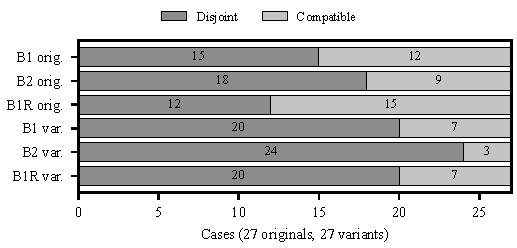
\includegraphics[width=\columnwidth]{build/figures/labels.pdf}
\caption{Predicted labels per model arm on the \NOriginals{} originals and \NVariants{} variants (counts; not accuracy).
No arm predicted \emph{Unresolved conflict}, \emph{Valid override}, or \emph{Insufficient evidence}.}
\label{fig:labels}
\end{figure}

\textbf{Label-free comparison.} No model arm labeled any original or variant an unresolved conflict or a valid
override; every prediction was \emph{Compatible} or \emph{Disjoint} (Fig.~\ref{fig:labels}), while B0 flagged
\BZeroCalledConfAnn{} of the 54. The challenge-oriented retrieval thus surfaced lexically similar pairs that the models
judged non-conflicting. The arms differ on the boundary between compatibility and condition-limited applicability: on
originals B2 chose \emph{Disjoint} \BTwoDistOrigDisjoint{} times and B1 \BOneDistOrigDisjoint{} times; B1 and B2
agreed on \AgreeBOneBTwoOrigSame{} of 27 originals (Cohen's $\kappa = \AgreeBOneBTwoOrigKappa$) and
\AgreeBOneBTwoVarSame{} of 27 variants ($\kappa = \AgreeBOneBTwoVarKappa$). The first non-determined original on which
they disagree (by the declared selection rule) pairs a root rule ``use \texttt{Protocol} for decoupling'' with a nested
rule ``avoid \texttt{TYPE\_CHECKING}'', both Python-specific, for a TypeScript target. B1 treated both rules as
inactive; B2's extraction found no explicit condition and returned \emph{Compatible}. Which reading is right is a
judgment about implicit applicability that P1 does not settle and that human labels must resolve.

\textbf{Stability and sensitivity (RQ3).} Swapping only the order of the two instructions changed the label in four of
\NControls{} controls for each model arm (\BOneOrderStable{}, \BTwoOrderStable{}, and \BOneROrderStable{} unchanged for
B1, B2, and B1R), although all \NPDCtrl{} determined controls stayed correct. All \NVarTarget{} target-path variants,
which move the target out of the nested file's directory, were labeled \emph{Disjoint} by every arm; the label differed
from the original's in \BOneTVChanged{} (B1), \BTwoTVChanged{} (B2), and \BOneRTVChanged{} (B1R) cases, because many
originals were already judged inactive by condition. Placement variants changed B2's label \BTwoPVChanged{} time and
B1's \BOnePVChanged{} times out of \NVarPlacement{}; without reference labels we cannot say which changes are correct.

\textbf{Cost.} No arm had a failure, retry, or malformed output. B2 averaged \BTwoCallsPerCase{} calls and
\BTwoMeanOut{} output tokens per case, against \BOneCallsPerCase{} and \BOneMeanOut{} for B1; the equal-call control B1R
(\BOneRMeanOut{} tokens) changed its first answer in \BOneRReviewChanged{} of 81 cases. Latency is not compared because
the GPU was shared with another process for part of the runs.
\else\textbf{Pending.} \PendingReason\fi

\section{Threats to Validity}\label{sec:threats}
Without human labels, accuracy is measured only on the profile-determined subset, which B2 solves by construction and
which proved easy for the direct model; the semantic question of condition-based and implicit applicability remains
unmeasured, and agreement between methods is not accuracy. The sample is small (\NOriginals{} originals from
\NEvalReposWord{} repositories) and challenge-oriented, so it cannot estimate how often conflicts occur; the absence of
predicted conflicts may reflect the retrieval as much as the repositories. Tasks come from templates, and variants and
controls are constructed. Each arm ran once; despite a fixed seed, an exact repeat of B1's requests (B1R's first calls,
on the updated runtime) changed \RepeatDiffTotal{} of 81 labels, so differences of a few cases between arms or between
an original and its control are within run-to-run variation. One profile and one quantized open-weight model limit
generalization, and public repositories may appear in the model's training data. Results concern classification under P1, not whether agents follow instructions or produce
better code.

\section{Conclusion}\label{sec:conclusion}
\ifresultsCIPHER contributes a task definition, a traceable set of real AGENTS.md instruction pairs with controlled variants, and
a blinded annotation protocol. In this preliminary evaluation without human labels, a local open-weight model given the
full evidence resolved directory scope as reliably as a pipeline that computes it explicitly, and at lower cost, whereas
a scope-blind keyword heuristic raised false alarms; none of the mined pairs was judged a genuine conflict. The open
problem is condition-based and implicit applicability, where the methods disagree and an order swap alone alters some
predictions. Collecting independent human labels for those cases, and testing other models and loading profiles, are
the next steps.\else Pending.\fi

\section*{Acknowledgment}
Following IEEE policy~\cite{ieeeai}, we disclose AI assistance. OpenAI ChatGPT assisted with concept exploration,
literature synthesis, and drafting of the earlier proposal on which Sections~I--III build. Anthropic Claude (Opus 5.5,
via Claude Code) audited the related work against primary sources; wrote the software for sampling, case construction,
the annotation tool, the model arms, and the analysis; wrote the task templates, the annotation handbook, and the
practice items with their answers; performed the code and manuscript reviews; ran all experiments; and drafted the text
of every section, the tables, and the figure of this version under the authors' direction. No human annotation was performed for this
version, and no AI output was used as a reference label; the only reference is computed from file paths under P1.
Qwen3.6-35B-A3B is the system under evaluation. The authors reviewed the manuscript and are responsible for its content.

\bibliographystyle{IEEEtran}
\bibliography{refs}
